\begin{figure}[!h]
 \centering
 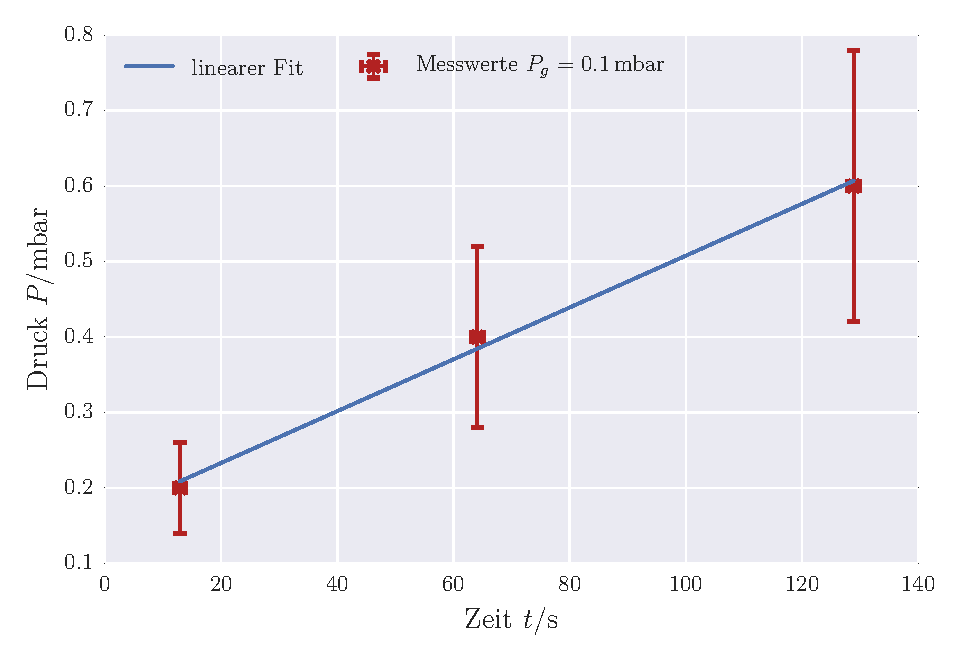
\includegraphics[scale=0.8]{../Grafiken/Leckrate_Drehschieber_0.pdf}
 \caption{Graphische Darstellung der Druckmesswerte in Abhängigkeit von der Zeit, aus der 1. Messreihe, und der
 	entsprechenden Ausgleichsgeraden. Der für die Messreihe eingestellte Gleichgewichtsdruck ist angegeben und als Messwert für $t=0$ mit eingetragen. Dieser ist grau dargestellt, da er für die 
 	Berechnung der Ausgleichsgeraden nicht verwendet wurde. \label{fig:leckrate_drehschieber_0}}
 \end{figure} 